\section{A Comparative Study of LMMs in Answering Visual Context Questions}
\label{app:LMMs_in_locality}

In our experiments, we evaluated numerous LMMs in answering visual context questions, such as Kosmos2, Fuyu-8B, and Qwen-VL-Chat. Our findings indicate that these models severely suffer from both hallucination and formatting errors when analyzing the scientific figures. Thus, we conclude that they lack the basic capabilities to generate valid rankings, which are crucial for calculating MRR.

\subsection{InternVL-Chat-1.1V}

\begin{table}[!t]
  \centering
  \small
  \begin{tabular}{lcc}
    \toprule
    \bb{Models} & \textbf{validation} & \textbf{test} \\
    \midrule
    Method 1 & 0.07 & 0.07 \\
    Method 2 & 0.218 & 0.186 \\
    Method 3 & 0.152 & 0.193 \\
    \bottomrule
  \end{tabular}
  \caption{MRR for InternVL}
  \label{tab:internvl_graular_result}
\end{table}

InternVL-Chat-1.1V operates with a short context window, a restriction that makes answering visual context questions particularly difficult. Although pairwise paper rankings were still possible within the token length restrictions, prompting the model with the entire list of possible reference paper titles and abstracts was not possible. Since the vanilla singular prompting method used to test other models with larger context windows (e.g. GPT-4V) on the visual context question dataset could not be applied to InternVL-Chat-1.1V, we used a slightly different prompting scheme. 

Three different ranking settings and methodologies were used to determine the rank of the reference paper for each visual context question. In the first setting, the model was repeatedly prompted to compare the true reference paper against each of the other papers one at a time in a head-to-head ranking. In this setting, we then considered the true reference paper's rank to be one more than the number of papers individually ranked higher than the true reference paper when compared side-by-side. In the second setting, the model was prompted to assign a rating to each of the sampled reference papers; the ratings were then sorted to generate a final ranking among the papers. Finally, in the third setting, the model randomly paired papers together, with each of the higher ranked papers in each pair considered to be ranked higher than every lower ranked papers. By then iteratively pairing papers among the set of higher-ranked papers and also iteratively pairing papers among all the initially lower-ranked ones, a ranking for the true reference paper was generated. 

Comparing each pair of sample papers requires a quadratic number of queries to the model, which requires a significant amount of time. Each of the three proposed methods, on the other hand, require a number of model queries that is linear in the total number of sample references. 

However, each of the methodologies have their own potential flaws. The first ranking methodology was asymmetric in that the true reference paper was prompted a different number of times; thus, for a method with no reasoning or retrieval capabilities, the true reference paper would have a $1/2^{n-1}$ chance of being ranked first, while it would have a $1/n$ chance of being ranked first in the ranking mechanism used in larger models, if there are $n$ papers to rank. Since MRR heavily favors smaller ranks, the first ranking methodology would bias the observed MRR downward. The second methodology, with zero-shot prompting, was unstable at times; furthermore, the model generally only chose from a set of a few possible ratings (i.e. $0$, $80$, $90$, or $100$ out of $100$), making it hard to differentiate and rank papers with the same rating. The third method is symmetric in its prompting but yields different results depending on initial pairings; we randomize the papers when pairing, and so this method is unbiased. We report the MRR values from the third method in Table \ref{tab:locality_mrr}. Detailed results are illustrated in Table \ref{tab:internvl_graular_result}. 


\subsection{Qwen-VL-Plus}
\label{appx:qwen-analysis}
In the visual context evaluation stage, only 53.1\% of Qwen-VL-Plus's rankings are valid, with a mere 5.0\% including the ground truth paper. 
MRR for QwenVL-Plus is evaluated based on 3 criteria: 
(1) \emph{Rank All}, assigning a zero value to any invalid rankings; 
(2) \emph{Rank Valid}, considering only valid rankings for MRR computation; 
and (3) \emph{Rank Ground Truth}, calculating MRR solely from rankings that include the ground truth. 
Detailed findings are presented in Table \ref{tab:qwenvl_breakdown}, though only \emph{Rank Valid} is reported in Table \ref{tab:detail_gpt_based}. Additional Error analysis can refer to Figure \ref{fig:qwen_locality1} below.

\begin{table}[!t]
    \centering
    \small
    \begin{tabular}{cccc}
    \toprule
    \textbf{model} & 
    \textbf{\begin{tabular}[c]{@{}c@{}}Rank \\ All\end{tabular}} & 
    \textbf{\begin{tabular}[c]{@{}c@{}}Rank \\ Valid\end{tabular}} & 
    \textbf{\begin{tabular}[c]{@{}c@{}}Rank \\ Ground Truth\end{tabular}}  \\
    (percentage) & & ($53.1\%$) & ($5.0\%$)\\
    \midrule
    QwenVL-Plus & 0.047 & 0.089 & 0.947 \\
    \bottomrule
    \end{tabular}
    \caption{MRR for QwenVL-Plus on the \emph{test} set across 3 evaluation settings.}
    \label{tab:qwenvl_breakdown}
\end{table}



% Commercial
\subsection{GPT-4V(ision)}
See Figure \ref{fig:gpt_locality1} and Figure \ref{fig:gpt_locality2} below.


\subsection{Claude-3-Opus}
See Figure \ref{fig:opus_locality1} and Figure \ref{fig:opus_locality2} below.


% qwen
\clearpage
\begin{figure*}[p]
    \centering
    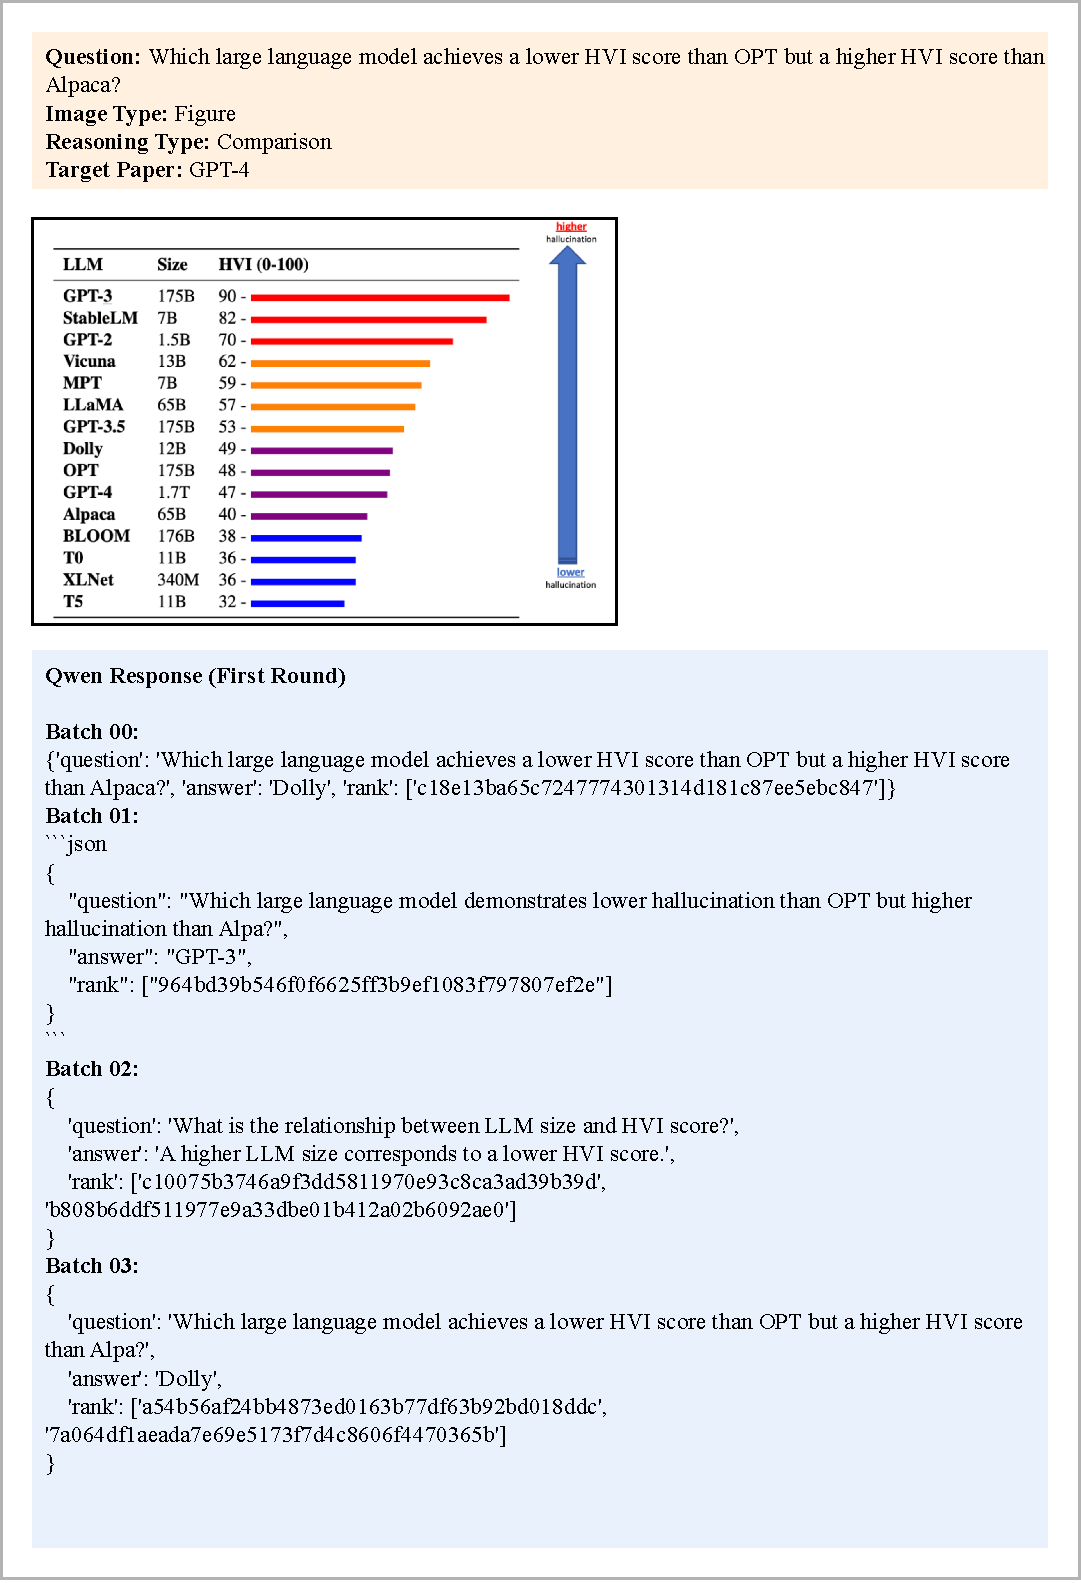
\includegraphics[width=\textwidth]{appx_figures/qwen_locality1.pdf}
    \caption{Qwen example output on visual context question - Part 1 of 3.}
    \label{fig:qwen_locality1}
\end{figure*}
\clearpage
\newpage
    
\begin{figure*}[p]
    \centering
    \ContinuedFloat
    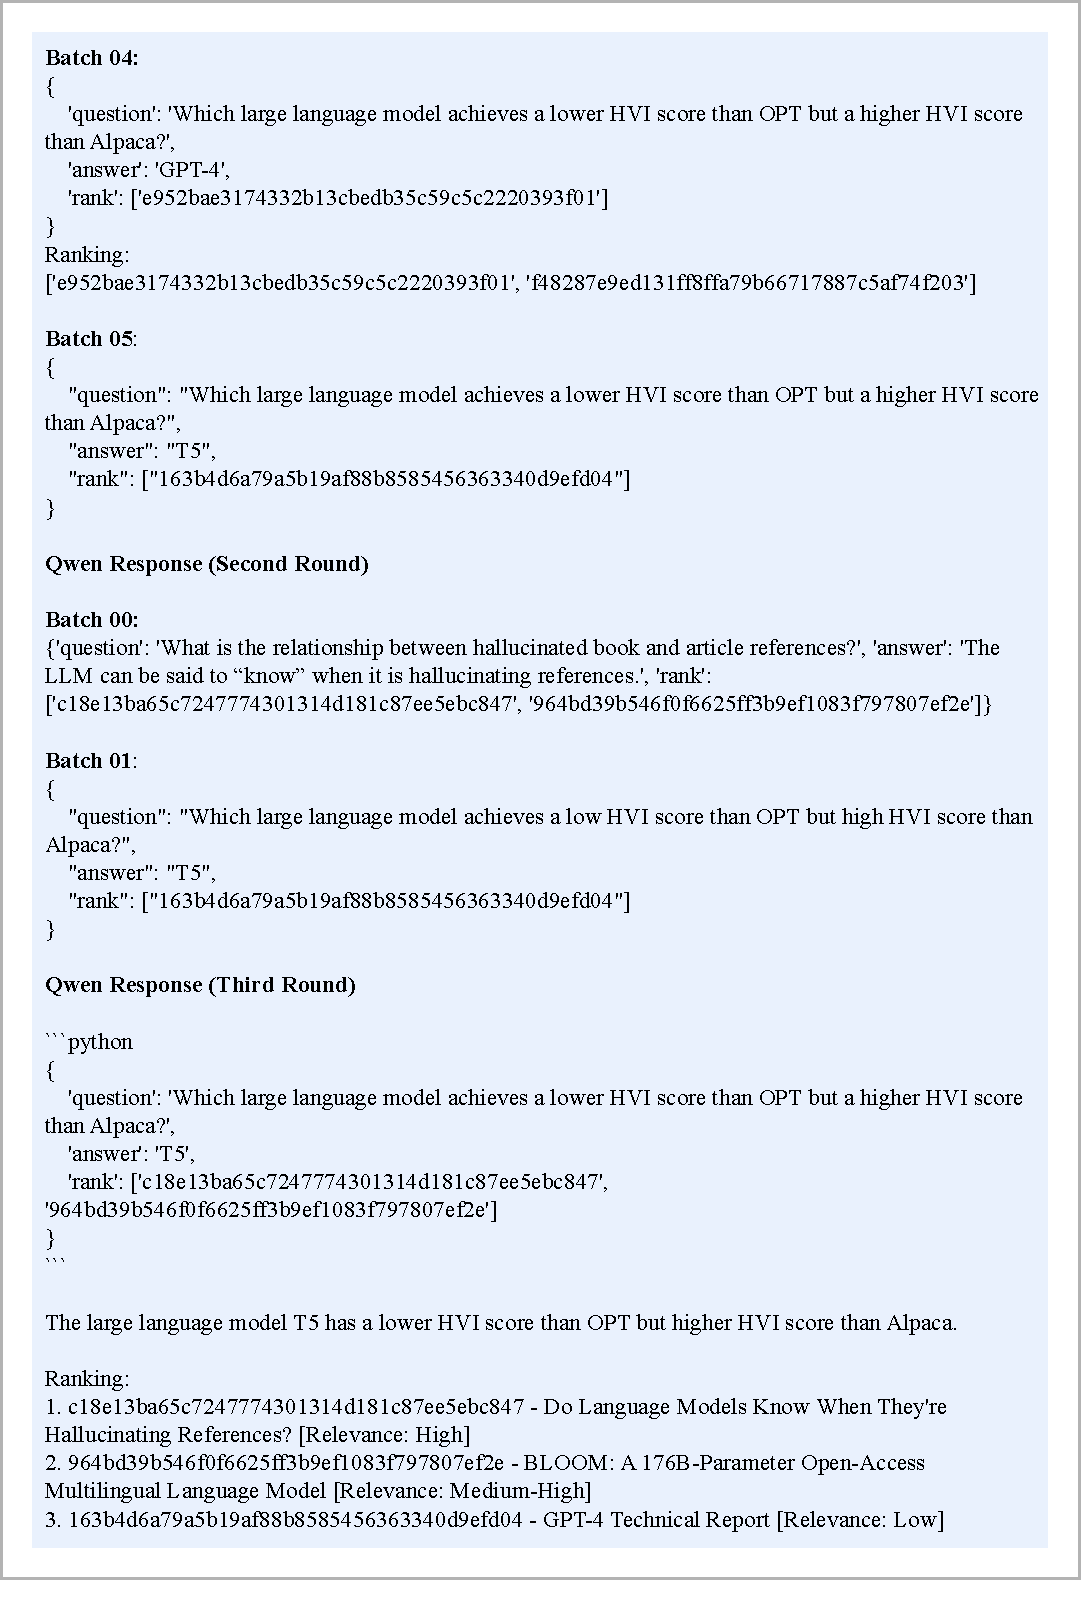
\includegraphics[width=\textwidth]{appx_figures/qwen_locality2.pdf}
    \caption{Qwen example output on visual context question - Part 2 of 3.}
    \label{fig:qwen_locality2}
\end{figure*}
\clearpage
\newpage
    
\begin{figure*}[p]
    \centering
    \ContinuedFloat
    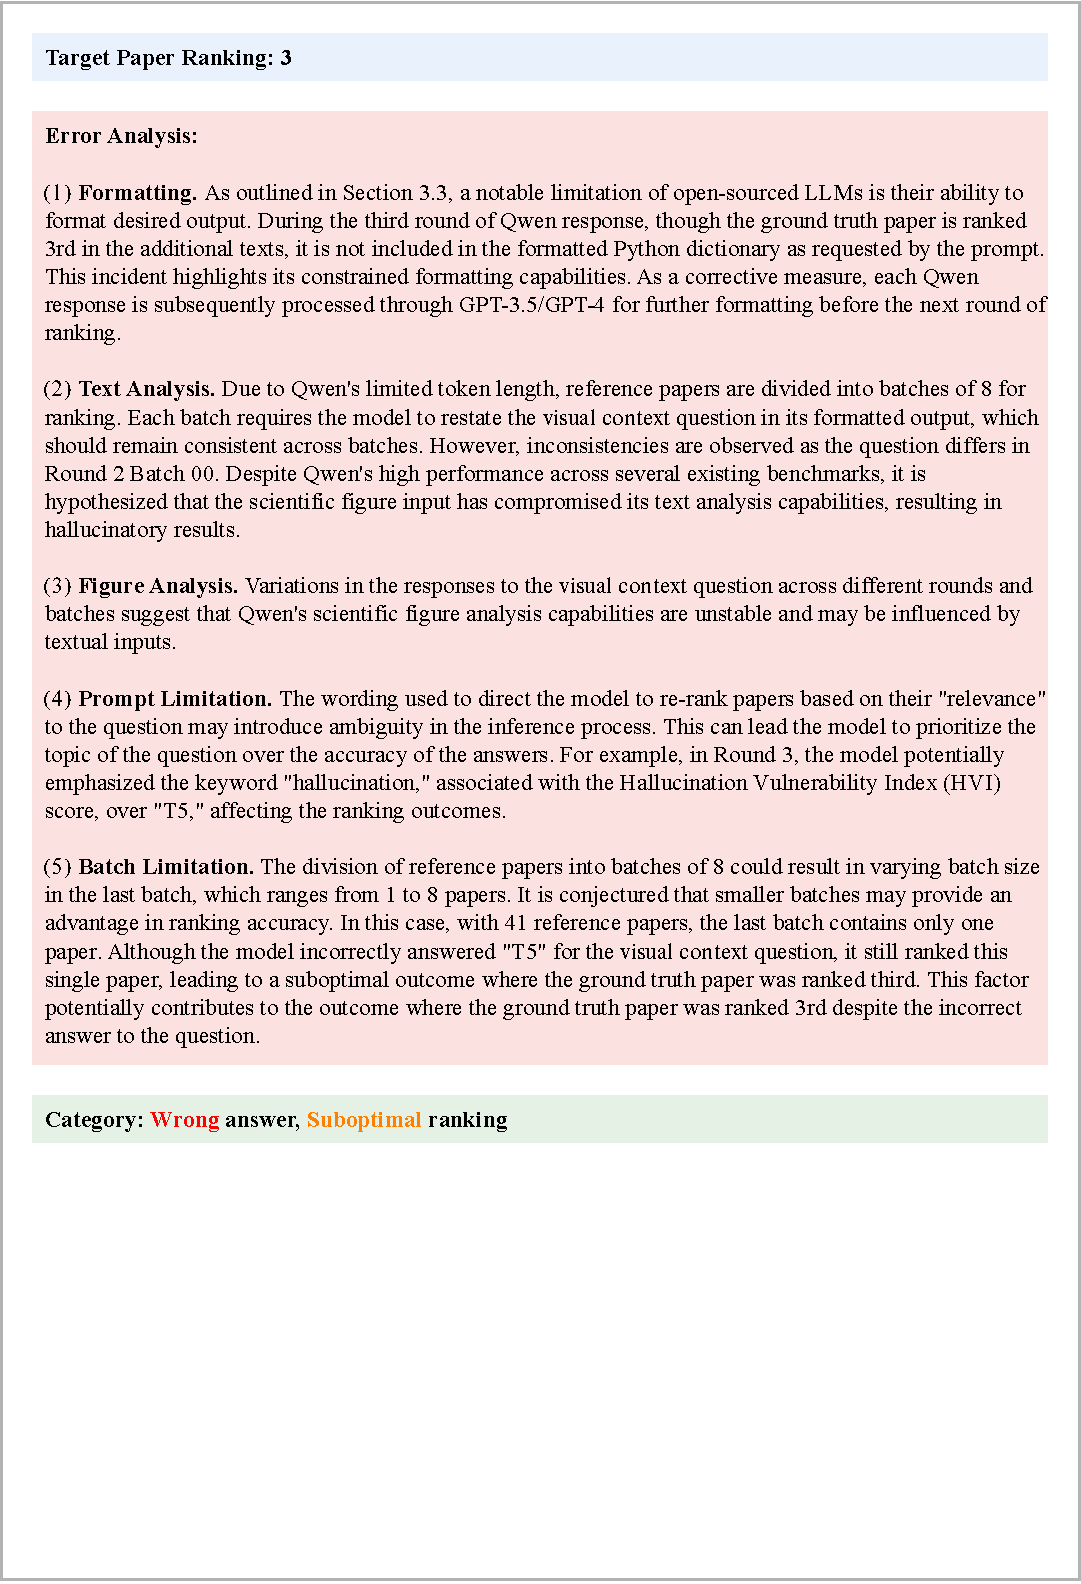
\includegraphics[width=\textwidth]{appx_figures/qwen_locality3.pdf}
    \caption{Qwen example output on visual context question - Part 3 of 3.}
    \label{fig:qwen_locality3}
\end{figure*}
\clearpage
\newpage


% gpt4vision
\begin{figure*}[p]
    \centering
    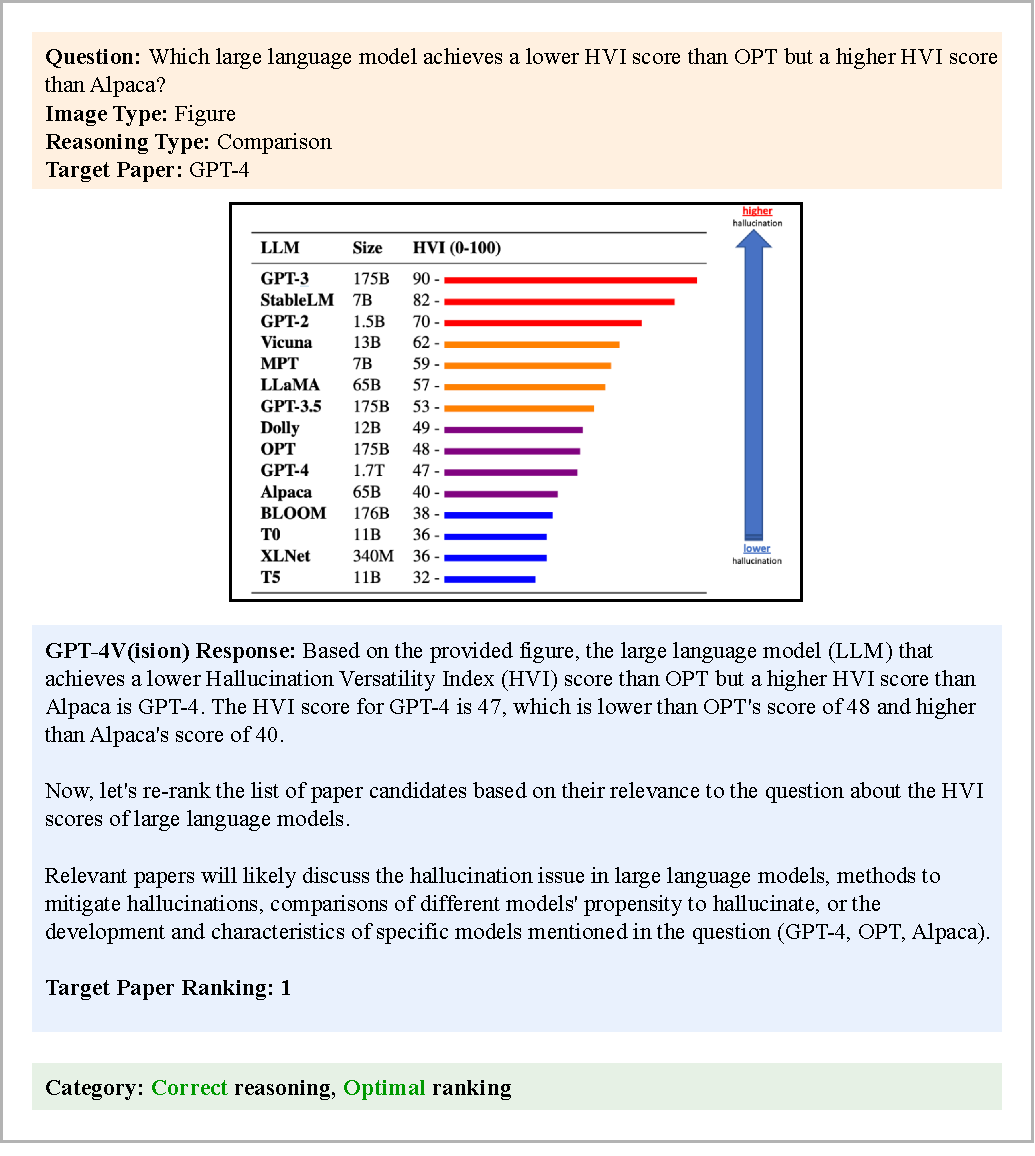
\includegraphics[width=\textwidth]{appx_figures/gpt4_locality1.pdf}
    \caption{GPT-4V(ision) example output 1 on visual context question.}
    \label{fig:gpt_locality1}
\end{figure*}
\clearpage
\newpage
\begin{figure*}[p]
    \centering
    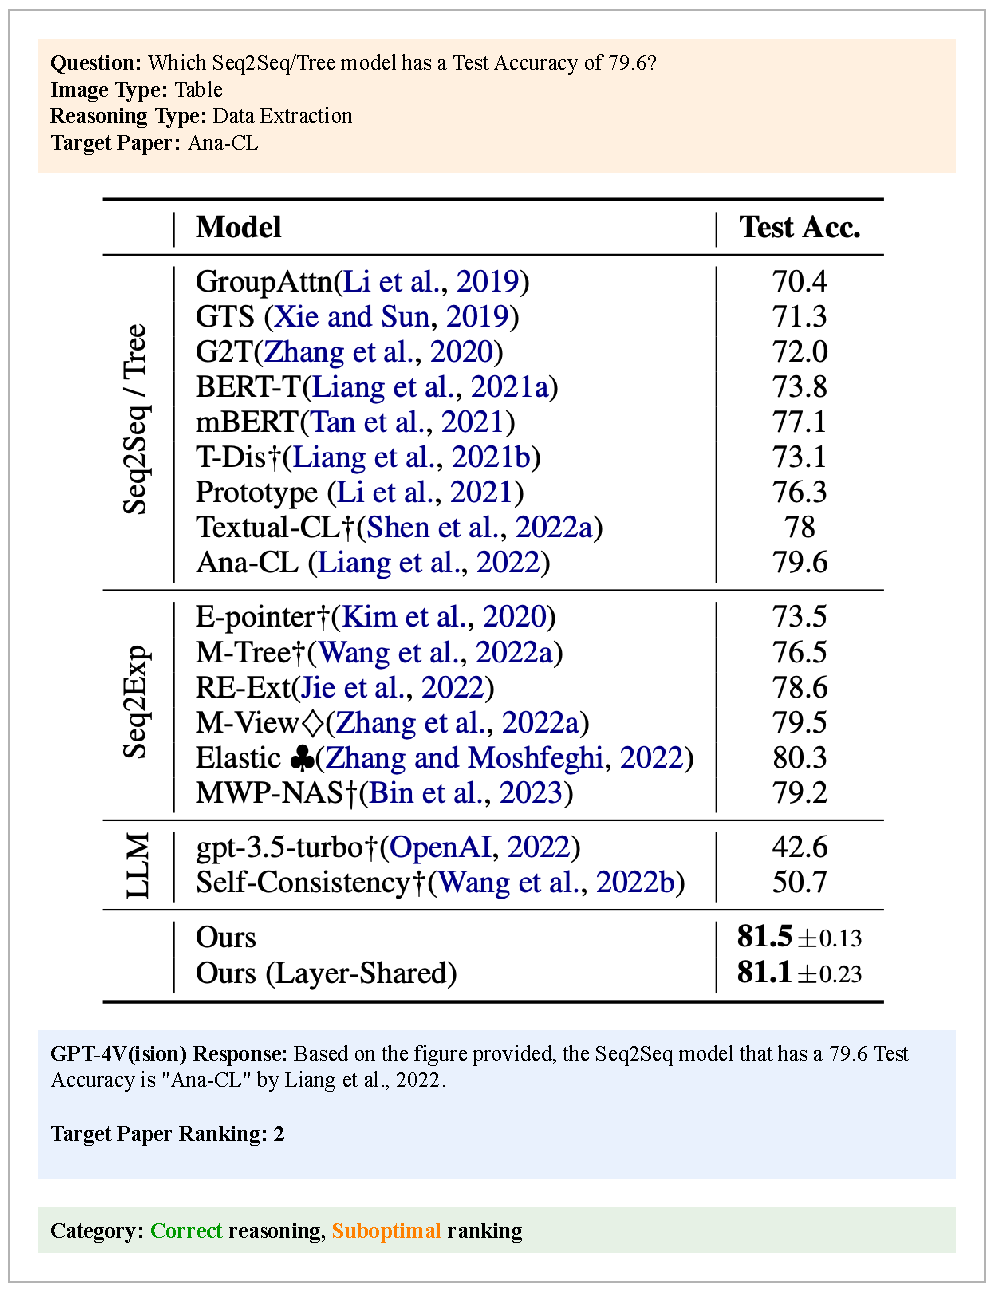
\includegraphics[width=\textwidth]{appx_figures/gpt4_locality2.pdf}
    \caption{GPT-4V(ision) example output 2 on visual context question.}
    \label{fig:gpt_locality2}
\end{figure*}
\clearpage
\newpage




% opus
\begin{figure*}[p]
    \centering
    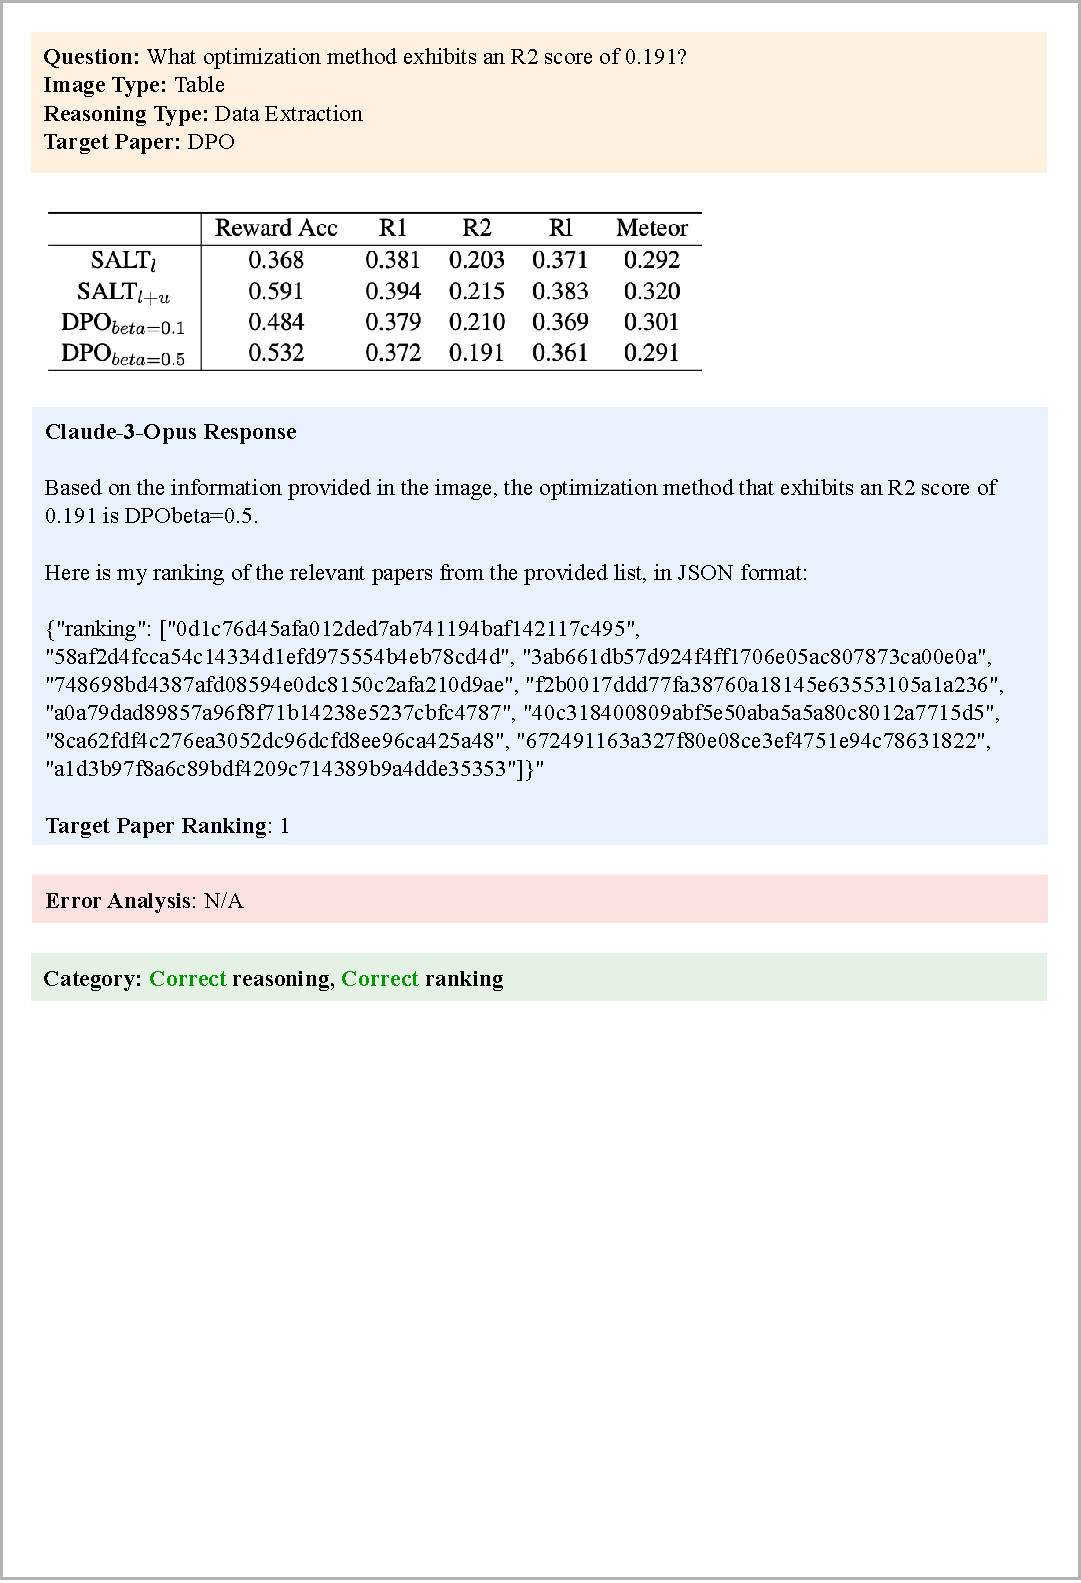
\includegraphics[width=\textwidth]{appx_figures/opus_locality1.pdf}
    \caption{Claude-3-Opus example output 1 on visual context question.}
    \label{fig:opus_locality1}
\end{figure*}
\clearpage
\newpage

\begin{figure*}[p]
    \centering
    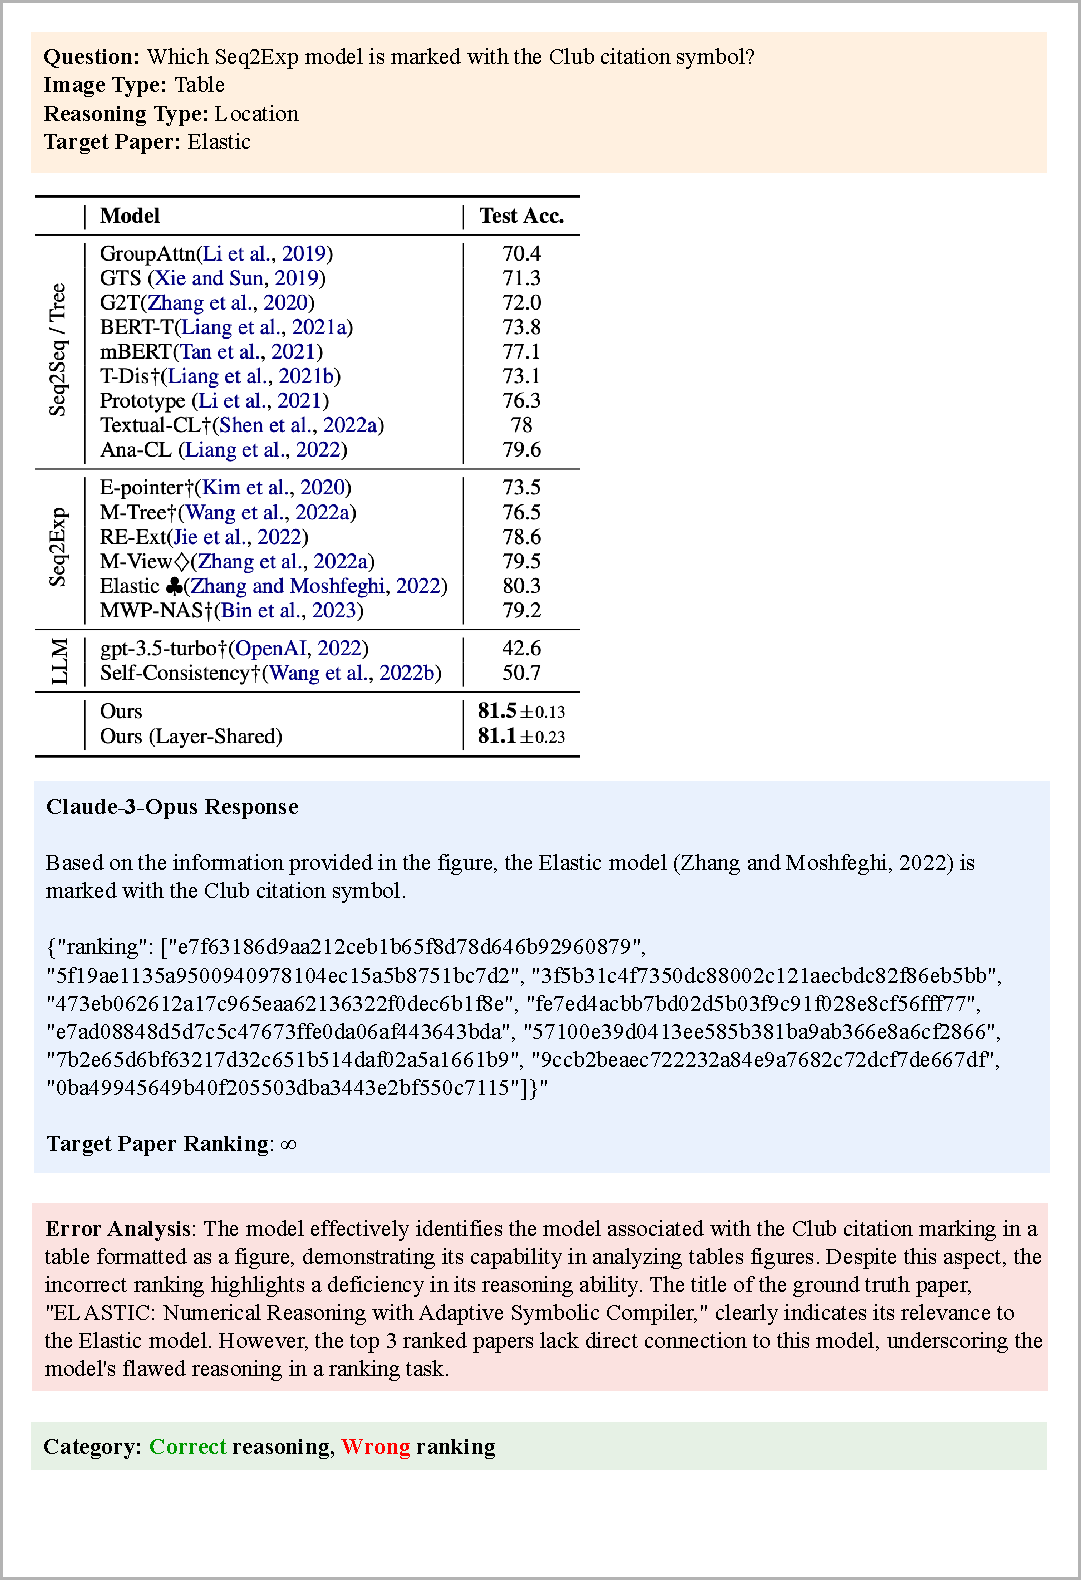
\includegraphics[width=\textwidth]{appx_figures/opus_locality2.pdf}
    \caption{Claude-3-Opus example output 2 on visual context question.}
    \label{fig:opus_locality2}
\end{figure*}
\clearpage
\newpage
